\documentclass[10pt]{article}

\input{../../utils/useful_packages}
\input{../../utils/short_notation}

\title{homework 2}

\date{\today}

\author{APC 523: Numerical Algorithm for Scientific Computing}

\hypersetup{
	pdftitle= {\@title},
	pdfauthor = {\@author},
	pdfsubject = {},
	pdfkeywords = {},
	pdfmoddate= {\@date},
	pdfcreator = {\@author},
	pdftoolbar=true,        
	pdfmenubar=true
}



\makeatletter
\def\@maketitle{
	\begingroup
	\centering
	{
		{\Large \MakeUppercase{\@title}\par}
		\vskip 0.1\baselineskip
		{\normalsize\noindent\@author\par}
		\vskip 0.1\baselineskip
		{\normalsize\noindent Due: Apr.20\par}
	}
	\endgroup
}
\makeatother

\titleformat{\section}{\Large}{\MakeUppercase{Problem} \thesection}{1em}{\MakeUppercase{#1}}

\begin{document}

\maketitle

\section{}

(a)

Define $f(x)\equiv 1$, which can be interpolated exactly, $f(x)=\sum_{j=0}^{N}f_jL_j(x)$.

Then $1\equiv f(x)=\sum_{j=0}^{N}f_jL_j(x)=\sum_{j=0}^{N}L_j(x)$


(b)

$$
L_j(x)=\frac{x-x_j}{x-x_j}\prod_{k=0,k\neq j}^N\frac{x-x_k}{x_j-x_k}=\frac{1}{x-x_j}\frac{\prod_{k=0}^N(x-x_k)}{\prod_{k=0,k\neq j}^N(x_j-x_k)}=\frac{w_j^{(N)}}{x-x_j}L^{(N)}(x)
$$

(c)
When $x\neq x_0,x_1,\cdots, x_N$,

$$
P_N(x)=\sum_{j=0}^{N}f_jL_j(x)=\sum_{j=0}^{N}f_j\frac{w_j^{(N)}}{x-x_j}L^{(N)}(x)=L^{(N)}(x)\sum_{j=0}^{N}\frac{w_j^{(N)}}{x-x_j}f_j
$$

When $x=x_k$, $P_N(x)=x_k$ to avoid dividing by zero.

\[  P_N(x)= \left\{
\begin{array}{ll}
L^{(N)}(x)\sum_{j=0}^{N}\frac{w_j^{(N)}}{x-x_j}f_j & x\neq x_0,x_1,\cdots, x_N\\
f_k & x=x_k\\
\end{array} 
\right. \]


(d)

From part (a), it can be shown that 

$$
1\equiv \sum_{j=0}^{N}L_j(x) = \frac{w_j^{(N)}}{x-x_j}L^{(N)}(x)
$$

(e)

See attachment

(f)

Take N = 20001, because by doubling N, the error does not change, which can be considered as max error.

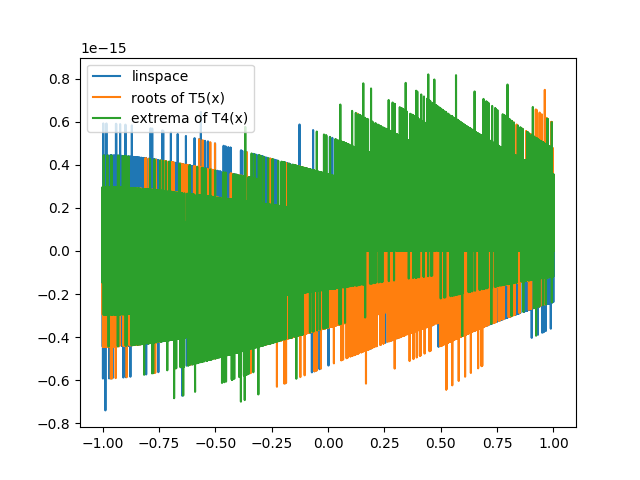
\includegraphics[width=4in]{p1f.png}

error of linspace: 7.400303277517389e-16

error of roots of T5(x): 7.477413297743957e-16

error of extrema of T4(x): 8.194533731269069e-16

\section{}

(a) and (b) see attachments

(c)

(i)

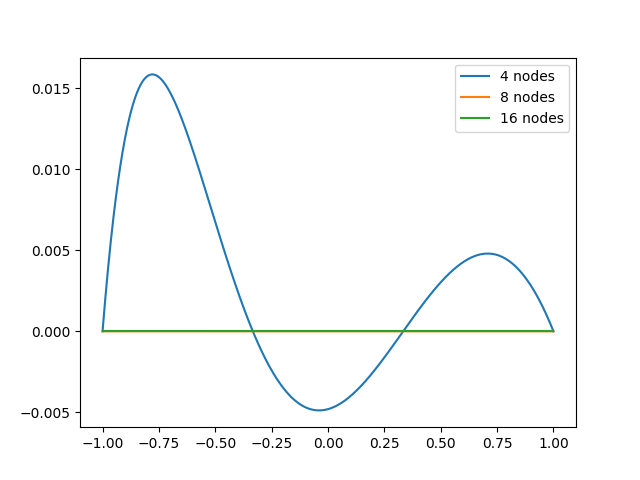
\includegraphics[width=4in]{p2ci.png}

error of 4 nodes: 0.015862018637759306

error of 8 nodes: 1.6274149425682455e-06

error of 16 nodes: 7.000836595671838e-14


(ii)

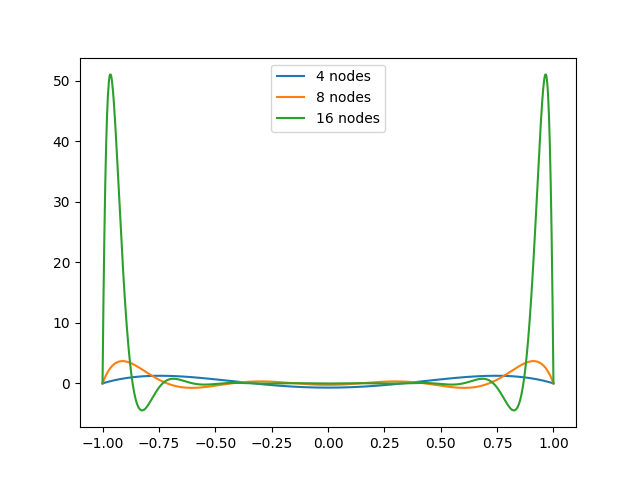
\includegraphics[width=4in]{p2cii.png}

error of 4 nodes: 1.2569071519343897

error of 8 nodes: 3.6792655802995706

error of 16 nodes: 51.07694738207374

(iii)

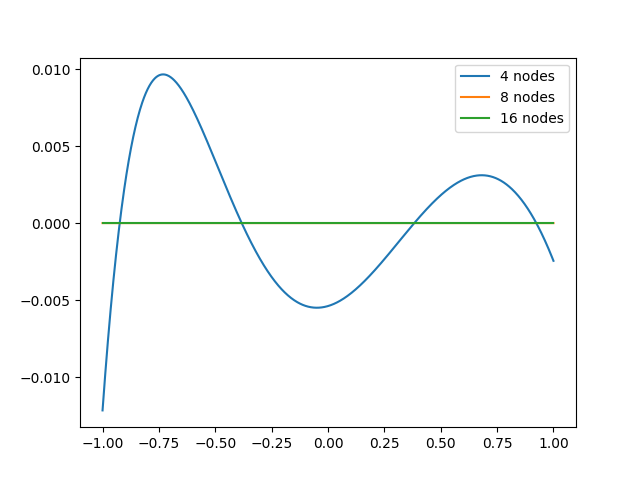
\includegraphics[width=3in]{p2ciii1.png}
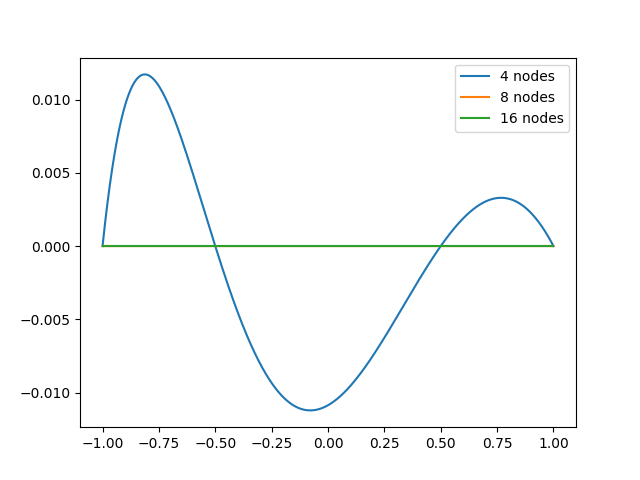
\includegraphics[width=3in]{p2ciii2.png}

chebyshev first kind (left): 

error of 4 nodes: 0.012157034328109002

error of 8 nodes: 4.843765068041292e-07

error of 16 nodes: 9.679389495585656e-16

chebyshev second kind (right): 

error of 4 nodes: 0.011716446906674694

error of 8 nodes: 5.275789099427979e-07

error of 16 nodes: 1.00776528914119e-15


(iv)

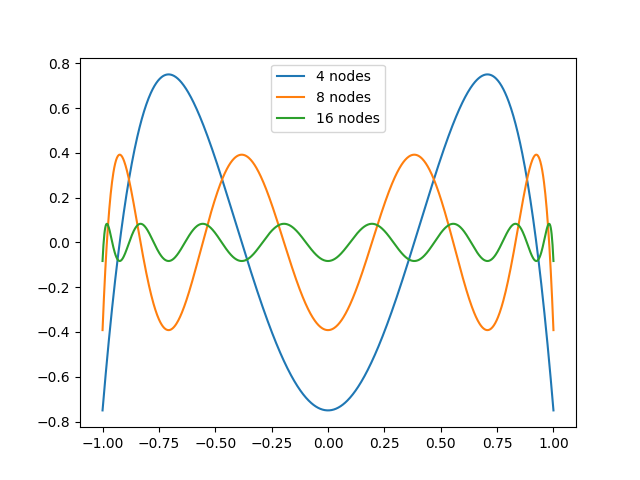
\includegraphics[width=3in]{p2civ1.png}
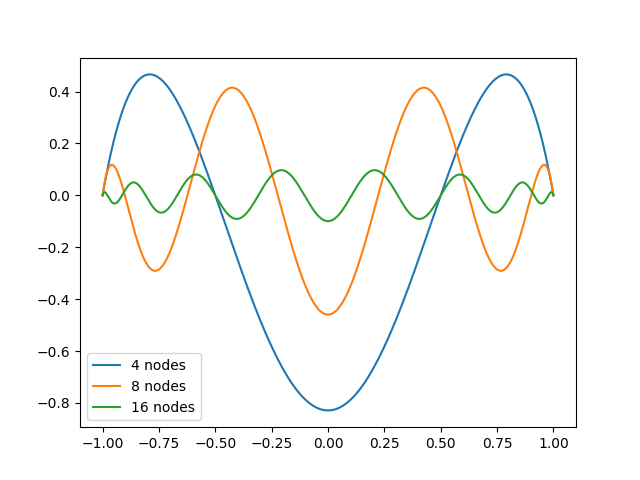
\includegraphics[width=3in]{p2civ2.png}

chebyshev first kind (left): 

error of 4 nodes: 0.7503001200480196

error of 8 nodes: 0.39174028459023014

error of 16 nodes: 0.08310704778474848

chebyshev second kind (right): 

error of 4 nodes: 0.8289124668435014

error of 8 nodes: 0.45960532477403604

error of 16 nodes: 0.09932185795194182

(d)

(i)

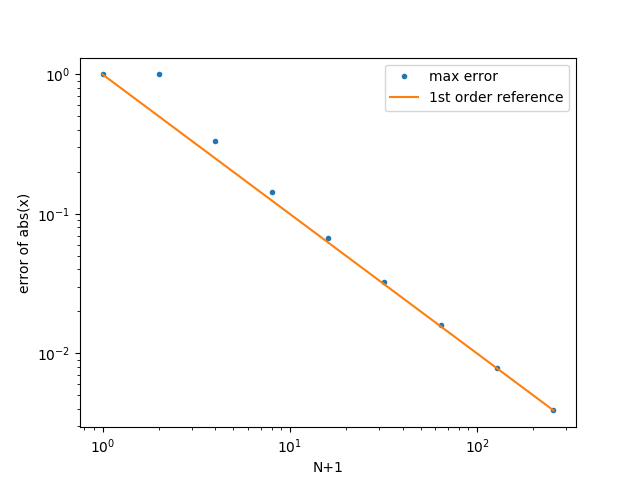
\includegraphics[width=2.2in]{p2di1.png}
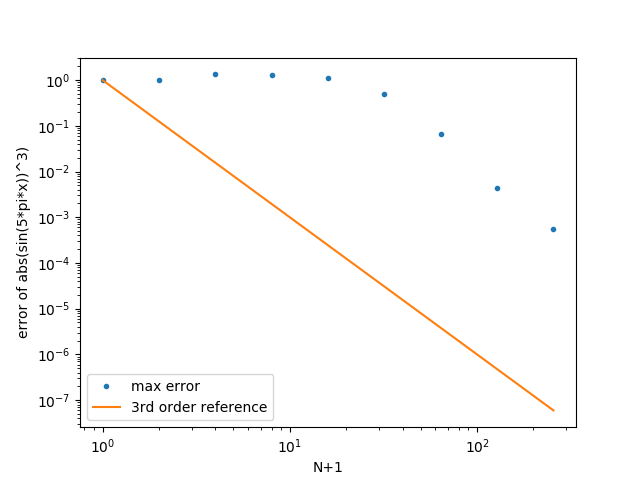
\includegraphics[width=2.2in]{p2di2.png}
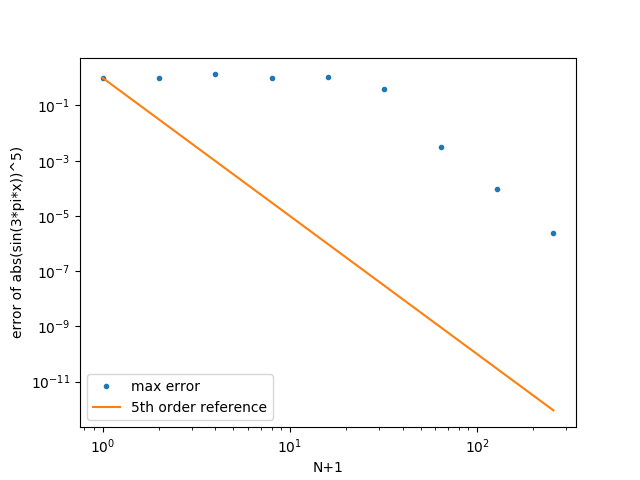
\includegraphics[width=2.2in]{p2di3.png}

(ii)

The plots are linear until it reaches machine precision.

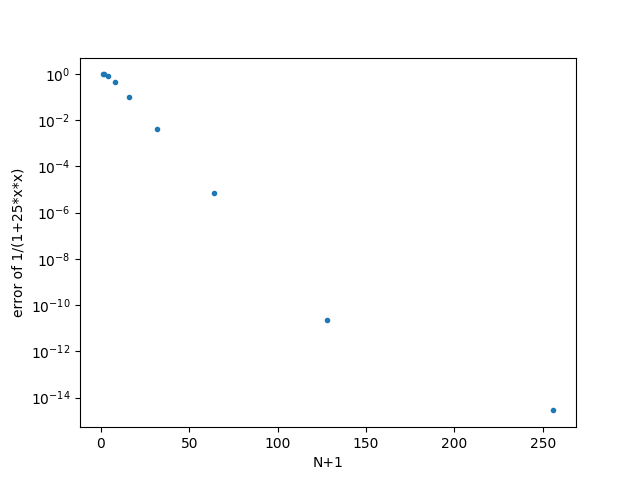
\includegraphics[width=2.2in]{p2dii1.png}
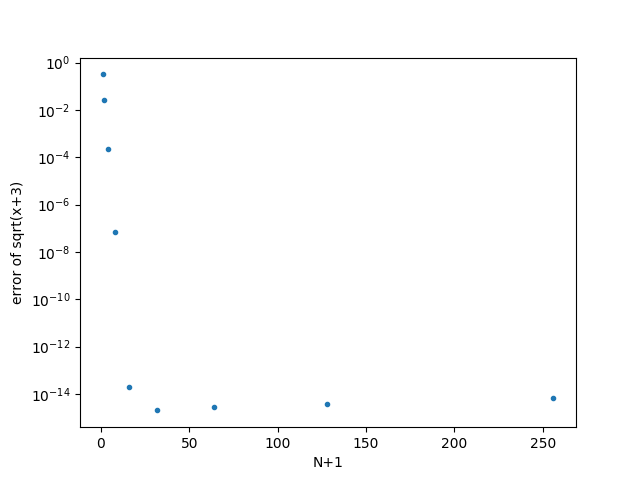
\includegraphics[width=2.2in]{p2dii2.png}
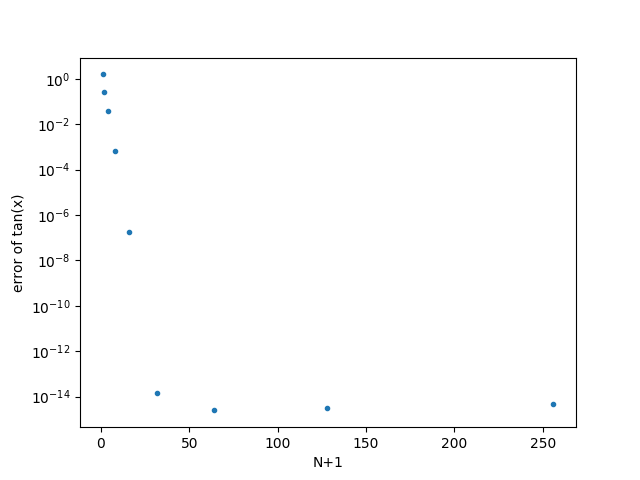
\includegraphics[width=2.2in]{p2dii3.png}

(iii)

The plots are linear until it reaches machine precision. The last has large error because the function is oscillating at high wavenumber.

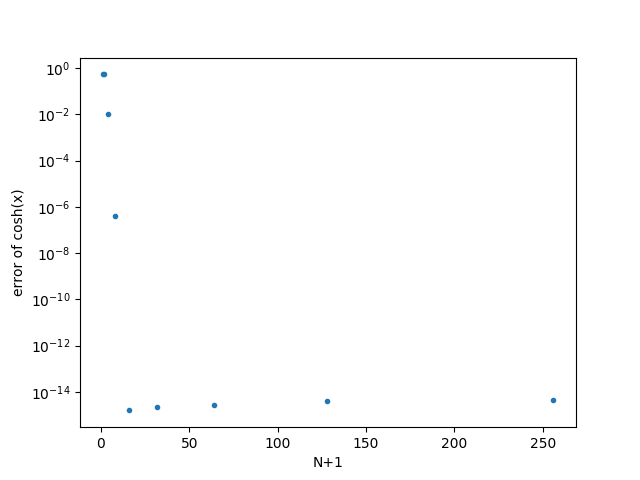
\includegraphics[width=2.2in]{p2diii1.png}
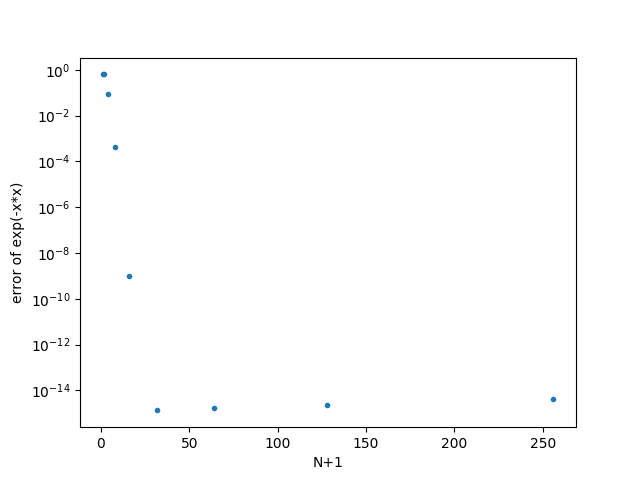
\includegraphics[width=2.2in]{p2diii2.png}
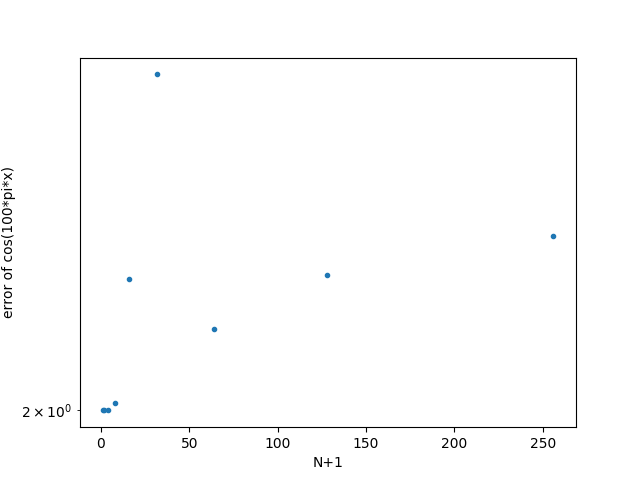
\includegraphics[width=2.2in]{p2diii3.png}


\section{}

(a) see attachment

(b)

(i) Write down several Chebyshev polynomials.

$$
T_0(x)=1, T_1(x)=x,T_2(x)=2x^2-1
$$
$$
T_3(x)=4x^3-3x, T_4(x)=8x^4-8x^2+1
$$

The power functions can be written as the linear combination of Chebyshev polynomials.

$$
1=T_0, x=T_1, x^2=\frac{T_2+T_0}{2}
$$
$$
x^3=\frac{T_3+3T_1}{4}, x^4=\frac{T_4+4T_2+3T_0}{8}
$$

The function $f(x)$ can be written as
$$
f(x)=5T_0+4T_1+5T_2+T_3+T_4
$$


(ii)

The result is [5. 4. 5. 1. 1.], which agrees with the theory.

(c)

It is found that $N=2^{17}-1$ is slower than $N=2^{17}$, which I think is because the even $N$ results in a complexity of $O(N\log N)$, while odd $N$ results in complexity of $O(N^2)$. Below is an output of time complexity.

N = 1023 , t = 0.00016951560974121094

N = 8191 , t = 0.053487300872802734

N = 8192 , t = 0.0007576942443847656

N = 131071 , t = 13.24022889137268

N = 131072 , t = 0.011487722396850586

(i)

Using timeit, and run number = 10 for N = $8,2^{13}-1,2^{13},2^{17}-1,2^{17}$, the runtime can be written down.

\begin{tabular}{cc}
\hline
N & time\\
\hline
8 & 0.0003882179989886936\\
$2^{13}-1$ & 0.5343649590031418\\
$2^{13}$ & 0.004654142001527362\\
$2^{17}-1$ & 133.21833001599953\\
$2^{17}$ & 0.0784644900013518\\
\hline
\end{tabular}

(ii)

The runtime with respect to N in a loglog plot can be shown, the runtime should be approximately 1st order.

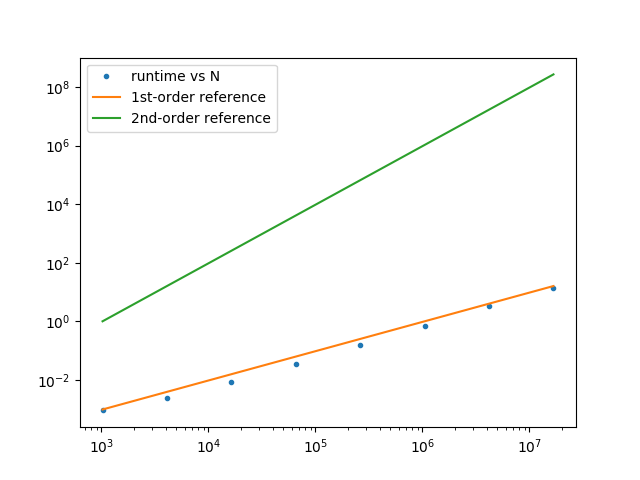
\includegraphics[width=4in]{p3cii.png}





\end{document}